\documentclass[11pt,fontset=none]{ctexart}

\usepackage[margin=0.82in]{geometry}
\usepackage{fontspec}
\usepackage{xcolor}
\usepackage{graphicx}
\usepackage{amsmath}
\usepackage{booktabs}
\usepackage{tabularx}
\usepackage{array}
\usepackage{enumitem}
\usepackage{float}
\usepackage[font=small,labelfont=bf,justification=raggedright,singlelinecheck=false]{caption}
\usepackage{xurl}
\usepackage{hyperref}
\usepackage{tikz}
\usetikzlibrary{arrows.meta, positioning, shapes.geometric, calc, fit, backgrounds}

\graphicspath{{figures/}}

\setmainfont{Latin Modern Roman}
\setCJKmainfont[
  BoldFont={Noto Serif CJK SC},
  ItalicFont={Noto Serif CJK SC}
]{Noto Serif CJK SC}
\setCJKsansfont[
  BoldFont={Noto Sans CJK SC},
  ItalicFont={Noto Sans CJK SC}
]{Noto Sans CJK SC}
\setCJKmonofont[
  BoldFont={Noto Sans CJK SC},
  ItalicFont={Noto Sans CJK SC}
]{Noto Sans CJK SC}

\definecolor{Ink}{HTML}{17202A}
\definecolor{Muted}{HTML}{5E6B73}
\definecolor{Blue}{HTML}{2563EB}
\definecolor{Teal}{HTML}{0F766E}
\definecolor{Green}{HTML}{15803D}
\definecolor{Amber}{HTML}{B7791F}
\definecolor{Red}{HTML}{B91C1C}
\definecolor{Panel}{HTML}{F6F8FB}
\definecolor{Line}{HTML}{CBD5E1}
\definecolor{SoftBlue}{HTML}{DBEAFE}
\definecolor{SoftTeal}{HTML}{CCFBF1}
\definecolor{SoftGreen}{HTML}{DCFCE7}
\definecolor{SoftAmber}{HTML}{FEF3C7}
\definecolor{SoftRed}{HTML}{FEE2E2}
\definecolor{SoftGray}{HTML}{EEF2F7}

\hypersetup{
  unicode=true,
  colorlinks=true,
  linkcolor=Blue,
  urlcolor=Teal,
  citecolor=Blue,
  pdftitle={以人为中心的实验室自主化：AR辅助实验、场景级学习与具身机器人集成},
  pdfauthor={Lachlan Chen, AgInTiFlow; AgInTi Lab, LazyingArt LLC}
}

\setlength{\parindent}{0pt}
\setlength{\parskip}{0.55em}
\setlist[itemize]{leftmargin=1.35em, topsep=0.2em, itemsep=0.1em}
\setlist[enumerate]{leftmargin=1.55em, topsep=0.2em, itemsep=0.1em}
\renewcommand{\arraystretch}{1.16}
\Urlmuskip=0mu plus 2mu
\emergencystretch=2em
\raggedbottom

\newcolumntype{Y}{>{\raggedright\arraybackslash}X}
\newcolumntype{L}[1]{>{\raggedright\arraybackslash}p{#1}}
\newcommand{\pill}[2]{%
  \tikz[baseline=(n.base)] \node[rounded corners=2pt, fill=#1, inner xsep=5pt, inner ysep=2pt] (n) {\footnotesize #2};%
}

\title{\vspace{-1.25cm}\textbf{以人为中心的实验室自主化}\\
\large AR 辅助实验、场景级学习与具身机器人集成}
\author{Lachlan Chen, AgInTiFlow\\AgInTi Lab, LazyingArt LLC\\\url{https://flow.lazying.art}}
\date{2026 年 6 月 6 日}

\begin{document}
\maketitle
\vspace{-0.8em}

\begin{center}
\makebox[\linewidth][c]{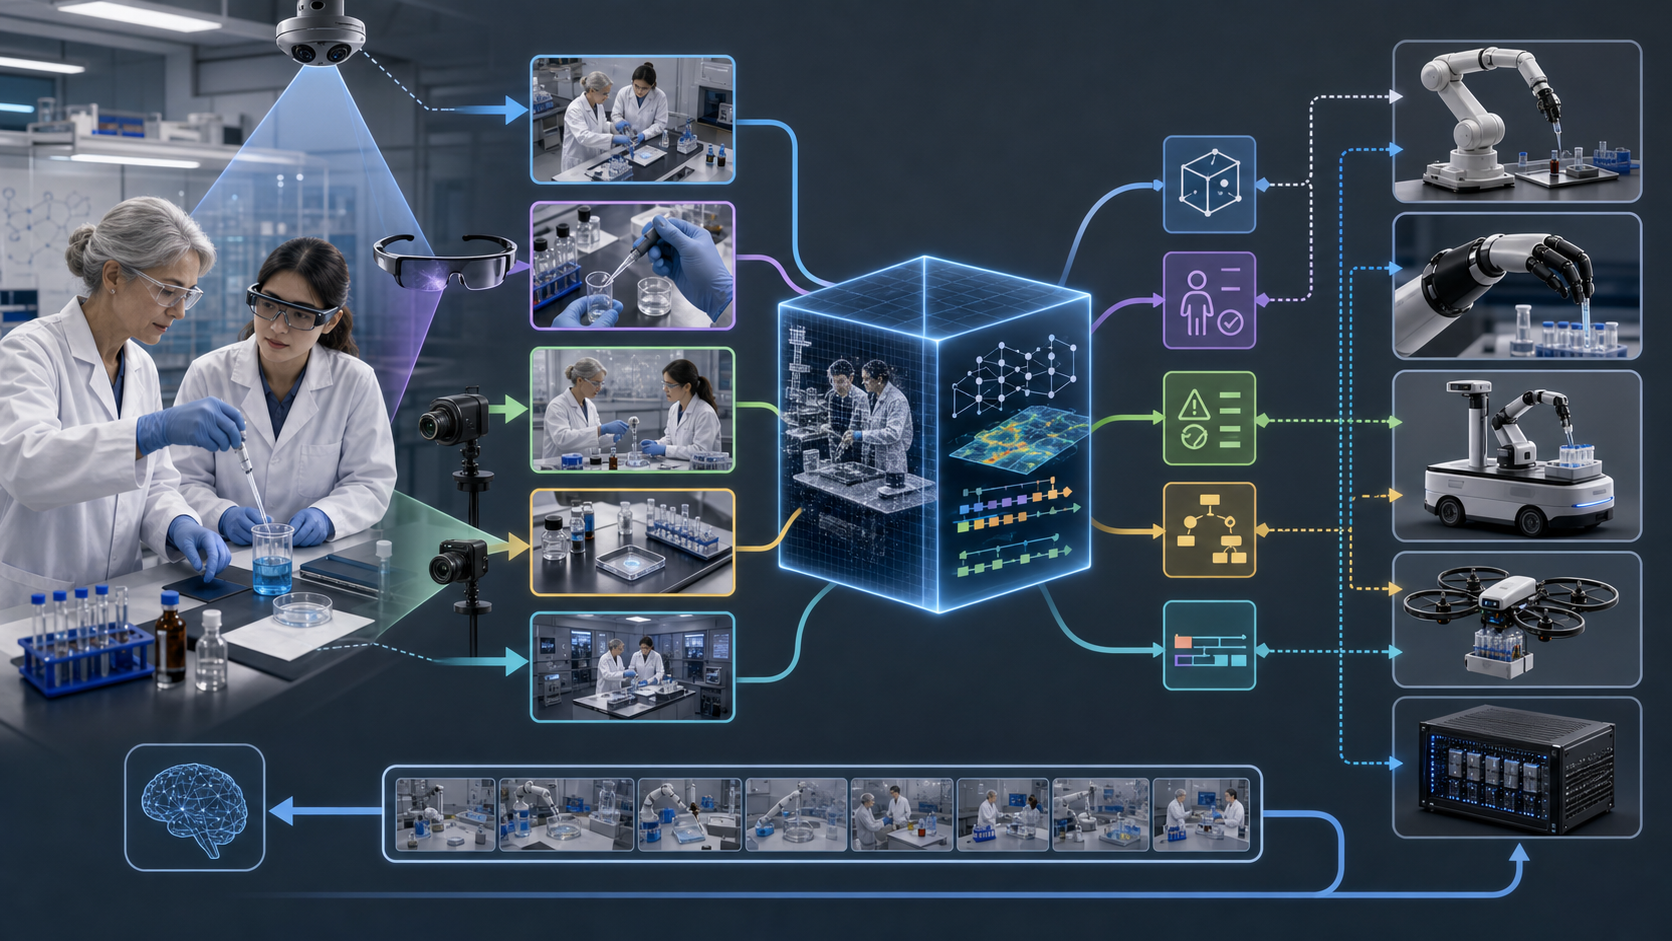
\includegraphics[width=1.08\linewidth,height=0.62\textheight,keepaspectratio]{scene_video_master_apprentice_training.png}}
\end{center}
\vfill
\newpage

\begin{abstract}
通向实用实验室机器人的最强路径，不是从第一天开始就复制完整的人体：仿生手、机械臂、眼睛、腿、移动底盘和人形外壳。更可行的路径，是把人类实验人员视为当前最通用的具身系统，并围绕人建立自主化栈：用 AR 眼镜做步骤引导，用摄像头做场景理解与质量控制，用机器人承担重复或危险动作，用共享 AI 模型从完整实验场景中学习。本文提出一种以人为中心的实验室自主化架构：第一阶段产品是 AR 与摄像头实验副驾驶；第二阶段产品是面向受限工作单元的机器人辅助层；长期产品是一个多具身操作系统，连接人、机器人手、机械臂、移动身体、无人机、固定仪器与 AI 推理。
\end{abstract}

\tableofcontents
\newpage

\section{执行论点}

如果目标是复现人的手、臂、眼睛、身体和脚，首先应该问的问题是：为什么不直接使用人？答案并不是机器人已经是更好的通用实验员。它们还不是。真正的答案是：人和机器人拥有不同的比较优势。人类仍然更擅长灵活感知、临场调整、隐性判断和异常恢复。机器人在工作重复、危险、可追踪、耗时、高频，或者物理边界足够清晰、可以被规范与验证时，才真正有价值。

因此，产品方向不应是“用人形机器人替代科学家”，而应是“把实验室变成可观测、可教学、可执行的环境”。在这样的环境中，资深人员可以教新手，AR 眼镜可以降低工作记忆负担，摄像头可以形成结构化记录，机器人可以在系统理解场景、协议、风险和决策点之后，逐步接管有边界的动作。

\textbf{战略判断。} 近期切入点是 AR 引导实验与摄像头质量控制系统；中期切入点是复用同一场景图和协议引擎的受限机器人辅助工作单元；长期切入点是师徒式学习平台，其中示范被记录为同步的场景视频，而不仅是机器人关节轨迹。

\begin{figure}[htbp]
\centering
\resizebox{\linewidth}{!}{%
\begin{tikzpicture}[
  font=\sffamily,
  box/.style={rounded corners=5pt, draw=Line, very thick, align=center, minimum height=1.05cm, text width=3.6cm, fill=white},
  human/.style={box, fill=SoftGreen, draw=Green!70},
  robot/.style={box, fill=SoftBlue, draw=Blue!65},
  system/.style={box, fill=SoftTeal, draw=Teal!65},
  warn/.style={box, fill=SoftAmber, draw=Amber!70},
  arrow/.style={-{Latex[length=3mm]}, very thick, draw=Ink!72, shorten >=2pt, shorten <=2pt}
]
\node[human] (human) at (0,1.7) {人的优势\\\footnotesize 判断、灵巧、恢复、隐性协议知识};
\node[robot] (robot) at (0,-1.7) {机器人的优势\\\footnotesize 重复性、记录、耐力、危险隔离};
\node[system] (scene) at (5.0,1.7) {仪器化场景\\\footnotesize AR、摄像头、协议状态、对象状态};
\node[system] (policy) at (5.0,-1.7) {有边界的自主\\\footnotesize 已验证动作、安全门、异常路径};
\node[warn] (product) at (10.2,0) {可行产品\\\footnotesize 先做人类副驾驶，后做机器人执行};

\draw[arrow] (human) -- (scene);
\draw[arrow] (robot) -- (policy);
\draw[arrow] (scene) -- (product);
\draw[arrow] (policy) -- (product);
\draw[arrow, dashed] (scene) -- node[right, font=\footnotesize\color{Muted}] {数据引擎} (policy);
\end{tikzpicture}}
\caption{核心设计原则不是替代人，而是比较优势：人负责教学和恢复；机器人执行已验证任务；仪器化场景连接两者。}
\label{fig:comparative-advantage-cn}
\end{figure}

\section{为什么不要先做仿生人形实验员}

仿生实验员会把许多难题捆绑在一起：手部灵巧度、机械臂力控、主动视觉、导航、平衡、安全、工具使用、语义推理、化学兼容性、清洁、校准和协议理解。每个组件都可以单独演示，但如果集成系统无法在普通实验室中可靠完成真实协议，它就很难成为商业产品。

\begin{table}[htbp]
\centering
\small
\begin{tabularx}{\linewidth}{@{}L{2.55cm}Y Y@{}}
\toprule
\textbf{能力} & \textbf{人类基线} & \textbf{何时使用机器人} \\
\midrule
灵巧操作 & 能处理特殊物体、柔性判断、别扭台面布局和一次性恢复。 & 动作重复、可夹具化、可测量，并能由摄像头、天平、液位或仪器输出验证。 \\
视觉理解 & 能从混乱场景中推断意图、上下文、风险、缺失物品和模糊协议含义。 & 场景可以转为结构化状态：对象身份、位姿、容器状态、PPE 状态、步骤进度和异常标记。 \\
移动能力 & 能穿过现有实验室、开门、换工具，并适应杂乱环境。 & 移动平台的收益足以覆盖成本，或任务是库存、运输、巡检、跨仪器物流。 \\
责任归属 & 对判断、安全和偏差进行签署确认。 & 系统能记录每个动作、传感器值、异常、决策和人工覆盖。 \\
训练方式 & 资深人员通过示范、纠正和解释教新手。 & 示范能被记录为同步场景数据，并转为可复用的协议、感知和策略资产。 \\
\bottomrule
\end{tabularx}
\caption{人的身体是当前最通用的实验室具身系统。机器人应该从狭窄优势切入，而不是第一天就复制完整人体栈。}
\label{tab:human-robot-comparison-cn}
\end{table}

实际结论是：先从实验活动出发，而不是从机器人形态出发。机器人手只有在产品已经知道任务价值、失败形态、可用传感器和可靠的物理简化方式之后，才真正有用。

\section{为什么机器人仍然重要}

机器人仍然值得建设，因为实验室中确实存在不应永远由人工完成的工作。其价值在五类情况下最强。

\textbf{重复性。} 机器人可以在同一坐标系中，以同样的时间节奏和可记录参数，执行同一个已验证动作。这对样品制备、液体处理、孵育转移、成像准备和重复仪器上样很重要。

\textbf{耐力。} 机器人不会在夜间、周末或长筛选任务中疲劳。当瓶颈不是创造力而是持续执行时，工作单元可以持续运行。

\textbf{可追踪性。} 机器人动作或摄像头介导动作可以自动产生审计线索：对象身份、孔板图、试剂批次、转移体积、时间、图像、异常和操作者介入。自驱动实验室文献正在越来越强调指标、数据完整性和系统表征，而不是只强调“自主性”本身 \cite{volk2024metrics}。

\textbf{危险隔离。} 机器人可以把人从有毒试剂、重复劳损、气溶胶、高温、低温、辐射或污染风险中隔离出来。但安全必须被显式设计；近期自驱动实验室安全研究也指出，如果机器人没有被充分仪器化和约束，它们会引入新的危险 \cite{sdl2025safety}。

\textbf{数据生产。} 机器人也是数据生成器。每一次尝试、成功、失败和纠正，只要被标准化场景模型捕获，都可以转化为训练和流程改进数据。

\section{机器人演示与真实实验室应用之间的落差}

应用落差不只是模型智能问题，而是工作流特异性、安全、污染控制、夹具、校准、操作者信任、经济性和现有仪器集成共同作用的结果。许多机器人演示展示一个令人印象深刻的动作；实验室产品必须在可接受异常率下重复完成协议。

\begin{table}[htbp]
\centering
\small
\begin{tabularx}{\linewidth}{@{}L{3.0cm}Y Y@{}}
\toprule
\textbf{落差} & \textbf{为什么阻碍部署} & \textbf{实际应对} \\
\midrule
协议模糊 & SOP 常常省略隐性判断、视觉检查和异常规则。 & 把 SOP 转为步骤图，包含视觉前置条件、预期观察和升级路径。 \\
场景变化 & 容器、标签、仪器、光照、手部和遮挡都会变化。 & 使用校准固定摄像头加可穿戴视角；先构建实验室特定场景图，再做策略自主。 \\
操作可靠性 & 透明液体、软管、瓶盖、标签、手套和杂乱都会形成失败模式。 & 从可夹具化工作流开始，并增加液位、实验器具状态和完成检查摄像头。 \\
安全与合规 & 实验室要求 PPE、风险评估、化学卫生实践和人的责任归属。 & 把 AR 和机器人计划视为带安全门的辅助，而不是无边界自主。 \\
经济证明 & 通用机器人可能昂贵，却只节省少量时间片段。 & 先销售完成工作流的可靠性、减少返工、更快培训和更好记录，而不是硬件新奇性。 \\
\bottomrule
\end{tabularx}
\caption{可行性计划必须关闭部署落差，而不只是改进机器人模型。}
\label{tab:application-gap-cn}
\end{table}

\section{产品想法一：AR 辅助实验}

最快有用的产品是面向人工实验的 AR 引导。界面应该让实验像精确的游戏：下一个对象发光、目标区域高亮、正确动作被展示、计时器自动开始，系统通过摄像头和传感器验证完成情况。目标不是让操作者停止思考，而是移除不必要的记忆、搜索和记录负担，使操作者把注意力放在判断和安全上。

AR 有支持证据，也有设计警告。混合现实系统已经被探索用于化学工程实验室训练和劳动力发展 \cite{teixeira2023ar}。同时，化学 AR 学习研究显示，如果叠加信息设计不当，可能增加认知负荷 \cite{peeters2023ar}。因此，界面必须稀疏、上下文相关、以动作为中心。

\begin{figure}[htbp]
\centering
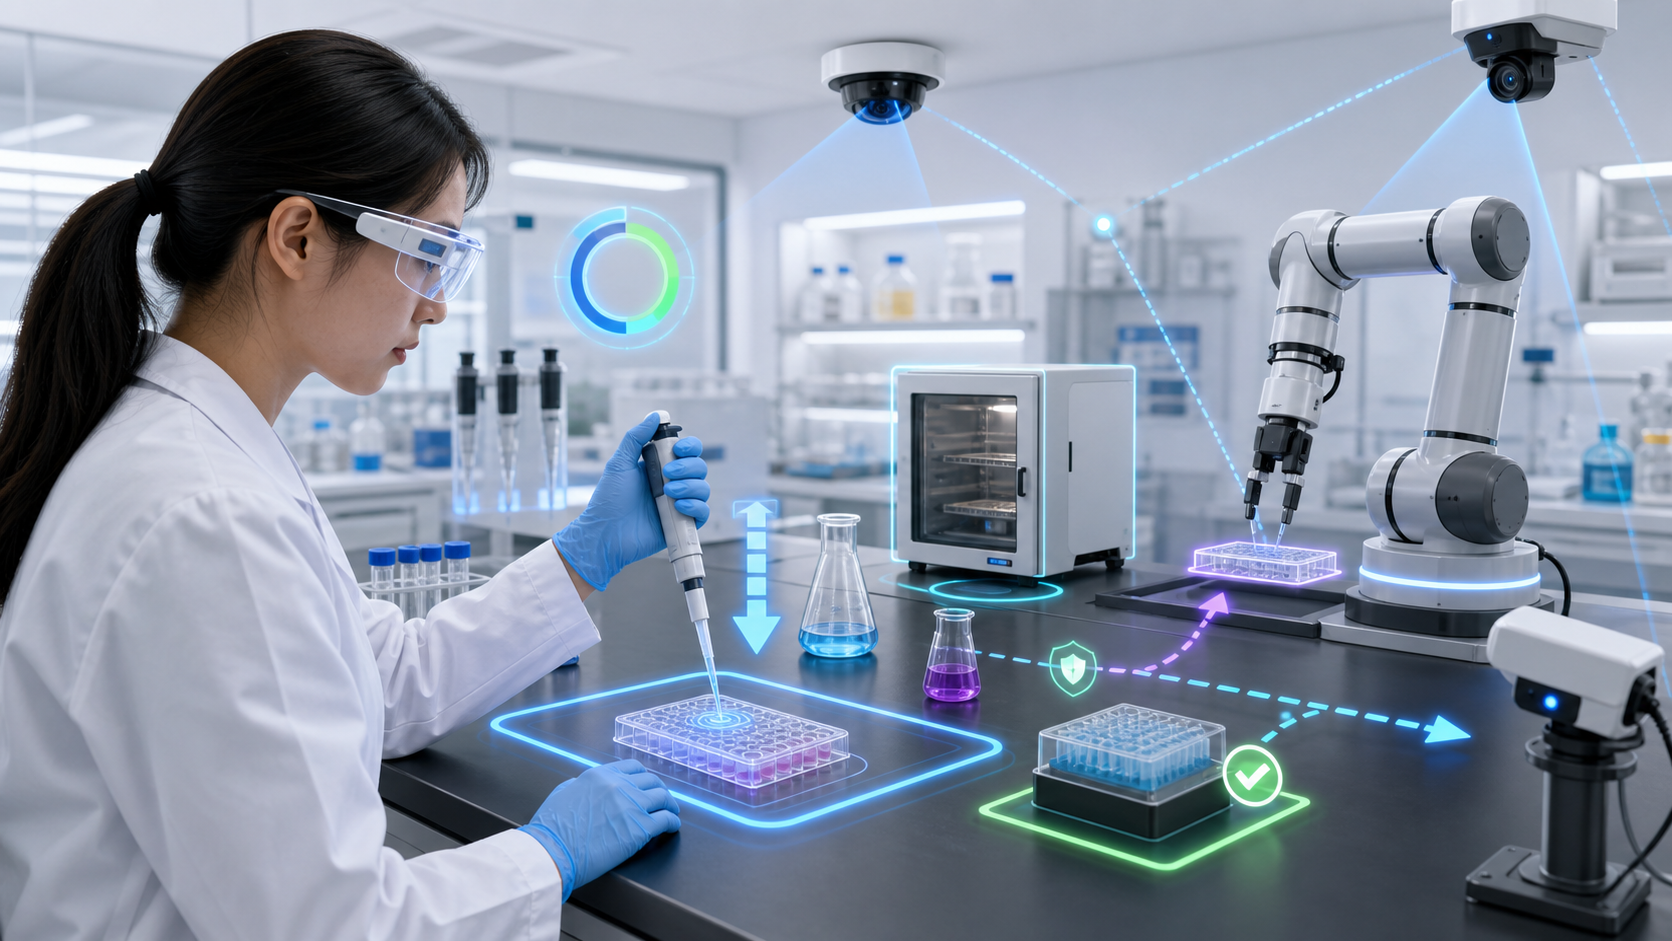
\includegraphics[width=\linewidth]{ar_guided_experiment_workflow.png}
\caption{AR 辅助实验概念。操作者看到空间提示、安全区域、进度标记和对象高亮；固定摄像头与机器人侧摄像头同时观察工作区，用于验证和后续机器人辅助。}
\label{fig:ar-guided-experiment-cn}
\end{figure}

\textbf{最小可行工作流。} 选择一个常见工作流，例如孔板移液、缓冲液配制、成像样品加载或仪器校准。把 SOP 编码为步骤图。每一步包含预期对象、位置、时间、视觉状态、可接受范围和失败恢复动作。

\textbf{操作者体验。} 操作者只看到当前步骤、相关对象和下一个物理目标。界面应避免大量文字。好的 AR 引导像驾驶舱：在恰当时间呈现刚好需要的信息。

\textbf{摄像头验证。} 摄像头层检查是否拿起正确对象、是否使用正确孔板区域、移液器方向是否合理、PPE 是否存在、预期状态变化是否发生。近期基于视觉的移液操作识别研究表明，RGB/深度采集、对象检测、姿态特征和时序模型可以识别标准与非标准操作 \cite{guo2026pipetting}。

\textbf{即时价值。} 这个产品可以在机器人开始动作之前，就减少培训时间、文档负担、偏差模糊性和重复错误。它同时生成未来机器人训练所需的数据引擎。

\section{产品想法二：摄像头优先的实验室 OS}

当前实验室已经包含大量隐性的视觉检查：人会观察颜色、浊度、液位、容器位置、移液器状态、孔板占用、仪器状态、清洁度、标签匹配和 PPE。摄像头优先的实验室 OS 把这些视觉检查转化为结构化数据。第一阶段不需要完整机器人自主。

\begin{figure}[htbp]
\centering
\resizebox{\linewidth}{!}{%
\begin{tikzpicture}[
  font=\sffamily\small,
  layer/.style={rounded corners=5pt, draw=Line, very thick, align=center, minimum height=1.05cm, text width=3.35cm, fill=white},
  sense/.style={layer, fill=SoftBlue, draw=Blue!65},
  state/.style={layer, fill=SoftTeal, draw=Teal!65},
  act/.style={layer, fill=SoftGreen, draw=Green!65},
  guard/.style={layer, fill=SoftAmber, draw=Amber!75},
  arrow/.style={-{Latex[length=3mm]}, very thick, draw=Ink!72, shorten >=2pt, shorten <=2pt}
]
\node[sense] (cams) at (0,2.1) {固定摄像头\\\footnotesize 顶视、台面、仪器视角};
\node[sense] (glasses) at (0,0) {AR 眼镜\\\footnotesize 第一人称视频、凝视、语音、姿态};
\node[sense] (instruments) at (0,-2.1) {仪器数据\\\footnotesize 日志、读数、警报、时间戳};

\node[state] (scene) at (4.7,1.05) {场景图\\\footnotesize 对象、位置、人员、工具、危险};
\node[state] (protocol) at (4.7,-1.05) {协议状态\\\footnotesize 步骤、前置条件、证据、异常};

\node[guard] (safety) at (9.2,2.05) {安全门\\\footnotesize PPE、危险、碰撞、授权};
\node[act] (ar) at (9.2,0) {人工引导\\\footnotesize AR 提示、纠正、检查表};
\node[act] (robot) at (9.2,-2.05) {机器人辅助\\\footnotesize 有界动作、交接、恢复};

\draw[arrow] (cams) -- (scene);
\draw[arrow] (glasses) -- (scene);
\draw[arrow] (instruments) -- (protocol);
\draw[arrow] (scene) -- (safety);
\draw[arrow] (scene) -- (ar);
\draw[arrow] (protocol) -- (ar);
\draw[arrow] (protocol) -- (robot);
\draw[arrow] (safety.east) -- ++(0.55,0) |- (robot.east);
\end{tikzpicture}}
\caption{摄像头优先的实验室 OS。第一个软件产品不是机器人“大脑”，而是共享的场景和协议状态，用于指导人并安全约束机器人辅助。}
\label{fig:camera-os-cn}
\end{figure}

这一方向已有多类近期案例支持。计算机视觉已经用于化学后处理的实时监控和控制，包括液位、浊度、均匀性、固体、残留和颜色 \cite{elkhawaldeh2024eye}。OT2Eye 使用 Opentrons OT-2 的图像和视频检测实验器具类型、位置和吸头状态 \cite{ot2eye2026}。Chemist Eye 使用分布式 RGB、深度和红外摄像头以及 VLM，在自驱动实验室中监控 PPE、火灾危险和机器人安全决策 \cite{chemistEye2026}。

实际含义很简单：摄像头不是配件，而是连接人类工作、机器人工作、训练数据和可审计性的桥梁。

\section{产品想法三：用场景视频训练，而不是只训练手部轨迹}

传统机器人学习常常聚焦手、夹爪、关节状态或末端执行器轨迹。这些是必要的，但并不完整。实验室任务不只是一条手部路径，而是一个情境化决策过程：哪个样品、哪个工具、哪个步骤、哪个安全约束、哪个异常、哪个视觉证据、哪个指令和哪个恢复动作。

近期机器人研究已经指向相同方向。RT-2 把机器人控制建模为视觉-语言-动作问题，使视觉和语言预训练可以迁移到动作 \cite{rt2}。Open X-Embodiment 汇集多机器人和多技能数据，展示跨机器人经验迁移 \cite{openx}。DROID 强调在大量真实场景和任务中的多样化操作数据 \cite{droid}。OpenVLA 发布了基于大量真实机器人示范训练的开放 VLA 模型 \cite{openvla}。更新工作如 $\pi_{0.5}$ 和 Qwen-VLA 进一步指向异构数据、高层语义预测、机器人具身描述、人类第一人称示范和跨任务泛化 \cite{pi05,qwenvla}。

因此，本文提出场景优先的训练方法：

\begin{enumerate}
  \item 用同步固定摄像头、AR 眼镜第一人称视频、语音、可用凝视、仪器日志和最终结果数据，记录资深人员教新手的过程。
  \item 把过程切分为协议阶段、对象状态、操作者意图、安全检查点、动作选择、错误、纠正和完成证据。
  \item 训练场景模型回答以下问题：当前正在执行哪一步？现在重要的对象是什么？存在什么风险？什么证据确认完成？下一步应该是什么？
  \item 最后再训练机器人专用策略，使有边界的物理动作以场景模型为条件。
\end{enumerate}

\begin{figure}[htbp]
\centering
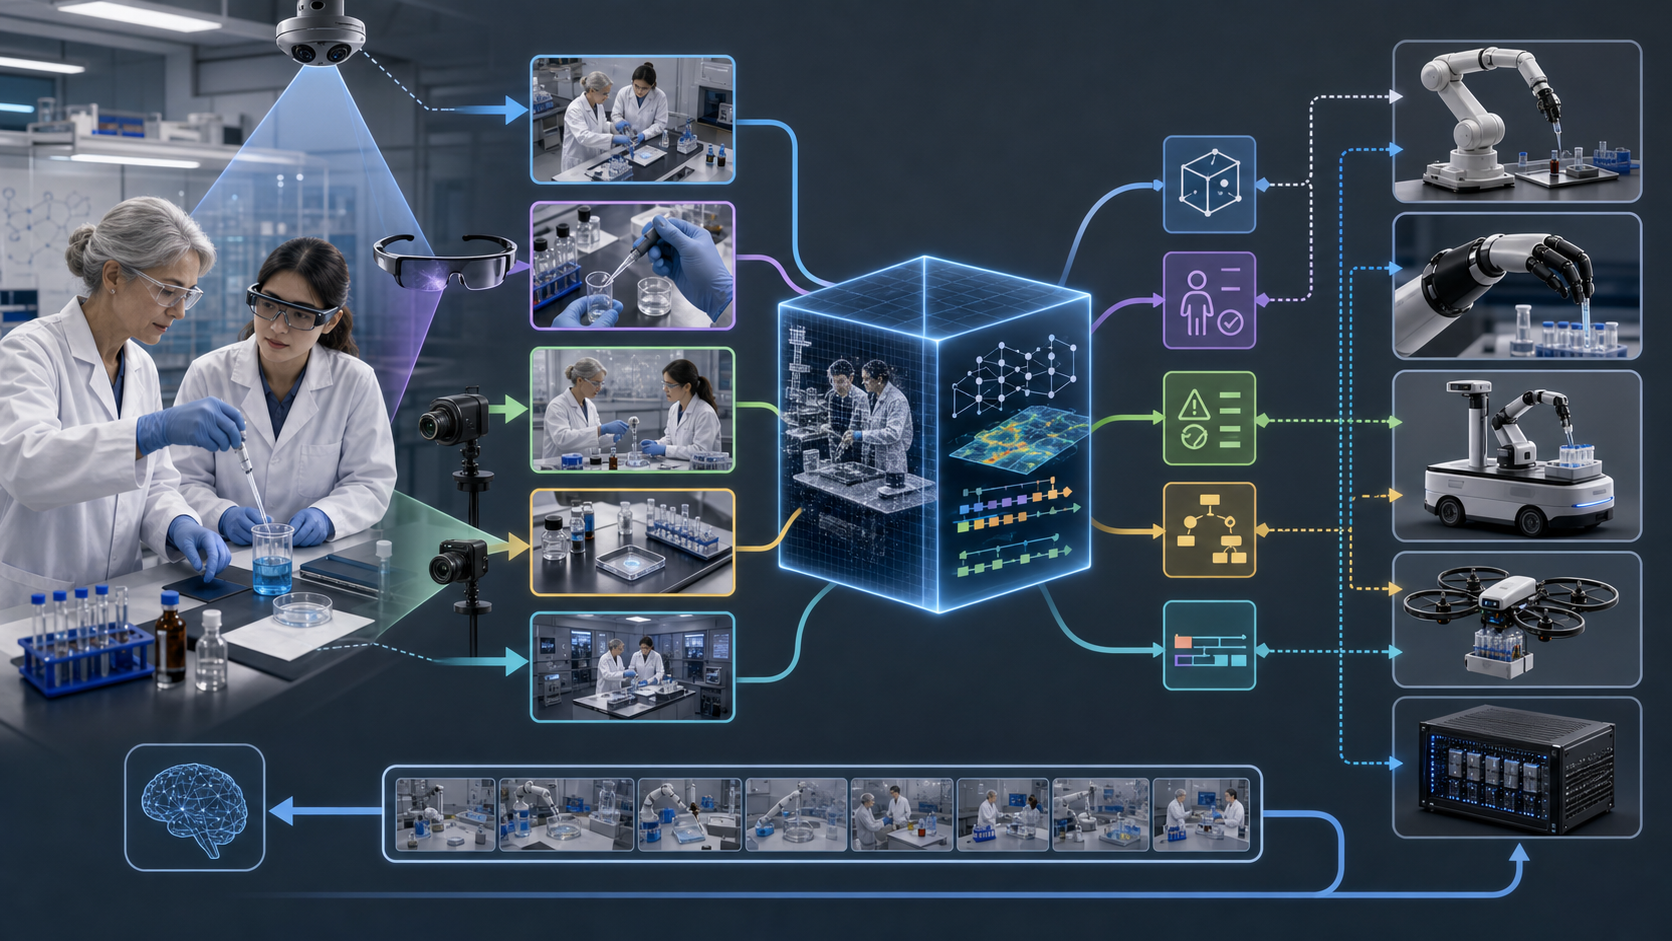
\includegraphics[width=\linewidth]{scene_video_master_apprentice_training.png}
\caption{师徒式场景视频训练概念。核心数据对象不仅是机器人轨迹，而是同步的人类示范、场景上下文、指令、纠正、安全状态和动作证据，之后可用于调度多种机器人具身。}
\label{fig:scene-video-training-cn}
\end{figure}

关键优势是迁移。如果系统理解场景和协议状态，机器人手、机械臂、移动身体、无人机或 AR 引导的人都可以被视为同一任务图的不同执行者。动作细节不同，但情境理解是共享的。

\section{师徒式学习循环}

资深人员教新手的模式是天然的数据引擎。资深人员已经在解释为什么某一步重要、要检查什么、可能出什么错、如何恢复。好的系统应该捕获这种教学信号，而不是丢弃它。

\begin{figure}[htbp]
\centering
\resizebox{\linewidth}{!}{%
\begin{tikzpicture}[
  font=\sffamily,
  stage/.style={rounded corners=5pt, draw=Line, very thick, align=center, minimum height=0.95cm, text width=2.9cm, fill=white},
  data/.style={stage, fill=SoftBlue, draw=Blue!65},
  model/.style={stage, fill=SoftTeal, draw=Teal!65},
  exec/.style={stage, fill=SoftGreen, draw=Green!65},
  eval/.style={stage, fill=SoftAmber, draw=Amber!75},
  arrow/.style={-{Latex[length=2.8mm]}, very thick, draw=Ink!72, shorten >=2pt, shorten <=2pt}
]
\node[data] (teach) at (0,0) {资深教新手\\\footnotesize 动作加解释};
\node[data] (capture) at (3.6,0) {同步采集\\\footnotesize 第一人称、外部视角、音频、仪器};
\node[model] (parse) at (7.2,0) {场景解析\\\footnotesize 对象、意图、风险、步骤状态};
\node[model] (policy) at (10.8,0) {策略库\\\footnotesize AR 提示和机器人动作};
\node[exec] (deploy) at (10.8,-2.0) {引导执行\\\footnotesize 人或机器人};
\node[eval] (qa) at (7.2,-2.0) {结果证据\\\footnotesize QC、偏差、完成};
\node[eval] (review) at (3.6,-2.0) {人工复核\\\footnotesize 批准、纠正、改进};

\draw[arrow] (teach) -- (capture);
\draw[arrow] (capture) -- (parse);
\draw[arrow] (parse) -- (policy);
\draw[arrow] (policy) -- (deploy);
\draw[arrow] (deploy) -- (qa);
\draw[arrow] (qa) -- (review);
\draw[arrow] (review) -- (capture);
\draw[arrow, dashed] (review) .. controls (1.0,-2.0) and (0.2,-1.1) .. (teach);
\end{tikzpicture}}
\caption{师徒式循环。每一次教学都会变成可复用资产：示范视频、解释、协议分段、安全标签、动作证据和纠正历史。}
\label{fig:master-apprentice-loop-cn}
\end{figure}

这个循环应被设计成产品，而不仅是数据采集项目。资深人员应能纠正步骤标签、批准建议规则、记录异常，并把一次示范标记为标准示范。新手应在每次复核示范之后得到更好的 AR 提示。机器人只有在场景状态和安全门已知时，才获得可执行动作。

\section{集成具身架构}

最终系统应连接 AI、人、机器人手、机械臂、移动底盘、无人机、固定摄像头、仪器和 AR 眼镜。架构不应假设每种具身都适用于每个协议，而应让每个具身暴露能力契约。

\begin{table}[htbp]
\centering
\small
\begin{tabularx}{\linewidth}{@{}L{2.35cm}Y Y@{}}
\toprule
\textbf{具身} & \textbf{有用角色} & \textbf{不应使用于} \\
\midrule
人类操作者 & 灵活处理、判断、异常恢复、教学示范、最终签署。 & 可廉价验证和自动化的高频重复步骤。 \\
AR 眼镜 & 步骤提示、视觉定位、免手持检查表、第一人称采集、语音备注、远程监督。 & 密集仪表盘、长文本，或遮挡 PPE、周边视野和安全意识的叠加层。 \\
固定摄像头 & 场景状态、实验器具检查、PPE 检查、液体与对象监控、审计证据。 & 没有治理与留存规则的私人区域或无边界录制。 \\
机器人手/臂 & 可夹具化操作、转移、孔板处理、仪器上样、重复准备。 & 未经人批准的开放式化学即兴操作或模糊操作。 \\
移动身体/脚 & 运输、库存、仪器间物流、巡检路线。 & 台面小工作流的第一产品，因为移动会增加成本而收益有限。 \\
无人机 & 在安全政策允许时做货架巡检、库存扫描、大型设施远程视觉检查。 & 湿台操作、对气流敏感的工作或拥挤人员区域。 \\
AI 模型 & 场景解析、协议状态、安全分诊、下一步建议、数据挖掘、策略选择。 & 危险或受监管步骤中的未经复核自主动作。 \\
\bottomrule
\end{tabularx}
\caption{具身应通过能力契约连接。系统根据当前步骤的成本、安全和可靠性，分配给最合适的执行者。}
\label{tab:embodiments-cn}
\end{table}

共享接口是协议-场景图。每个节点代表一种状态或动作：对象已检测、试剂已验证、PPE 存在、孔板已定位、液体已转移、孵育完成、读数已采集、异常已标记。人和机器人都读写同一张图，但权限不同。

\section{MVP 演示场景}

第一个公开演示应该选择一个真实实验室工作流：视觉上容易理解、可以安全重复运行，同时足够丰富，能展示 AR 眼镜、AI、机器人、无人机、摄像头和实验室环境为什么应该在同一系统中协同。一个强 MVP 是\textbf{AR 引导的样品接收与 96 孔板准备演示}，使用无危险彩色液体或低风险训练实验。演示不应试图证明完全自主，而应证明协调自主：每个执行者看到同一个协议状态，每个动作产生证据，系统在场景错误时可以停止或重定向工作。

\textbf{演示故事。} 一名新手操作者戴着 AR 眼镜进入实验室。AI 识别操作者、确认 PPE、加载协议，并高亮正确的试管架、孔板、移液器、试剂瓶和目标孔位。固定摄像头观察台面。无人机在密封货架或标记储存通道中进行短距离库存扫描，定位所需的封闭试剂盒；它不飞越开放液体、人员或活动台面。移动机器人或人类接收定位到的物品。操作者按照 AR 提示准备孔板。摄像头模型验证每个检查点。机械臂随后把封闭孔板移动到读板仪、孵育器或成像站。系统生成完整运行记录：协议步骤、对象证据、操作者确认、机器人动作、库存来源、偏差和最终结果图像。

\begin{figure}[htbp]
\centering
\resizebox{\linewidth}{!}{%
\begin{tikzpicture}[
  font=\sffamily\small,
  nodebox/.style={rounded corners=5pt, draw=Line, very thick, align=center, minimum height=1.0cm, text width=2.8cm, fill=white},
  human/.style={nodebox, fill=SoftGreen, draw=Green!65},
  sense/.style={nodebox, fill=SoftBlue, draw=Blue!65},
  ai/.style={nodebox, fill=SoftTeal, draw=Teal!65},
  robot/.style={nodebox, fill=SoftAmber, draw=Amber!75},
  outputbox/.style={nodebox, fill=SoftGray, draw=Ink!45},
  arrow/.style={-{Latex[length=2.8mm]}, very thick, draw=Ink!72, shorten >=2pt, shorten <=2pt}
]
\node[sense] (drone) at (0,2.0) {无人机库存扫描\\\footnotesize 密封货架、二维码标签};
\node[human] (ar) at (0,0) {AR 引导操作者\\\footnotesize PPE 检查、目标孔位};
\node[sense] (cams) at (0,-2.0) {固定实验室摄像头\\\footnotesize 台面、手部、孔板};

\node[ai] (scene) at (3.8,0) {AI 场景图\\\footnotesize 对象、位置、协议状态};
\node[ai] (gate) at (7.2,0) {安全与 QA 门\\\footnotesize 证据、偏差、权限};

\node[robot] (arm) at (10.7,1.05) {机械臂动作\\\footnotesize 封闭孔板转移};
\node[robot] (mobile) at (10.7,-1.05) {移动交接\\\footnotesize 耗材递送};
\node[outputbox] (record) at (14.1,0) {可审计运行记录\\\footnotesize 图像、时间戳、决策、结果};

\draw[arrow] (drone) -- (scene);
\draw[arrow] (ar) -- (scene);
\draw[arrow] (cams) -- (scene);
\draw[arrow] (scene) -- (gate);
\draw[arrow] (gate) -- (arm);
\draw[arrow] (gate) -- (mobile);
\draw[arrow] (arm) -- (record);
\draw[arrow] (mobile) -- (record);
\end{tikzpicture}}
\caption{MVP 演示流程。第一个演示应展示 AR 引导、摄像头 QA、AI 场景状态、无人机库存、机器人转移和完整实验记录之间的协调自主。}
\label{fig:mvp-demo-cn}
\end{figure}

\textbf{为什么这个场景强。} 观众容易理解，因为孔板、彩色孔位、AR 高亮、无人机货架扫描、机器人转移和最终孔板图像都是可见的。它安全，因为不需要危险化学品。它技术上诚实，因为人仍然执行灵巧湿实验步骤，而机器人只处理有边界的转移，无人机只处理库存观察。它商业上相关，因为培训、样品准备、库存、仪器上样和文档记录都是常见实验室痛点。

\begin{table}[htbp]
\centering
\small
\begin{tabularx}{\linewidth}{@{}L{2.45cm}Y Y@{}}
\toprule
\textbf{MVP 组件} & \textbf{首次演示角色} & \textbf{成功标准} \\
\midrule
AR 眼镜 & 告诉操作者拿什么、向哪里移液、何时等待、何时确认。 & 操作者不读纸质 SOP，也能更少犹豫地完成孔板。 \\
AI 场景模型 & 维护操作者、PPE、试管架、试剂、孔板、目标孔位、库存和仪器状态。 & 系统能解释当前步骤并识别下一个合法动作。 \\
固定摄像头 & 验证对象存在、手/工具位置、孔板位置和若干错误场景。 & 至少三个关键检查点能由视频证据验证。 \\
无人机 & 在密封货架或储存通道中扫描所需封闭试剂/耗材盒。 & 系统定位物品并更新场景图，且不进入湿台区域。 \\
机械臂 & 只移动封闭、可夹具化物品：孔板载具、封闭孔板或试管架。 & 机器人只在安全门批准后完成有边界转移。 \\
运行记录 & 合并 AR 确认、摄像头证据、无人机库存结果、机器人动作和最终图像。 & 运行结束时自动生成 PDF 或仪表盘条目。 \\
\bottomrule
\end{tabularx}
\caption{MVP 范围。每个组件都有可见角色和清晰通过/失败标准，避免演示变成模糊的机器人秀。}
\label{tab:mvp-scope-cn}
\end{table}

\textbf{演示中的失败时刻。} 演示应包含一个故意设置、可恢复的错误：把错误试管放进试管架、孔板旋转方向错误，或操作者伸向错误孔列。AR 叠加层应暂停步骤，摄像头模型应给出证据，机器人应拒绝下游转移，直到错误被纠正。这个时刻比完美脚本更能传达产品价值。

\textbf{构建目标。} MVP 不需要通用人形机器人。最小硬件是一台 AR 设备或平板替代、两个固定摄像头、一台带孔板夹具的小机械臂、一台被限制在标记库存路线或安全笼中的室内无人机，以及一台运行协议状态服务的工作站。软件目标是一个协议、一张场景图、一个可复核运行记录和五个可靠检查：PPE 存在、正确试管架、正确孔板方向、正确目标区域、允许封闭孔板转移。

\section{可行性路线图}

可行路径应分阶段推进。不要从人形机器人开始。先让人的工作可观测、结构化、更容易执行；再只自动化已有证据证明值得自动化的步骤。

\begin{table}[htbp]
\centering
\scriptsize
\begin{tabularx}{\linewidth}{@{}L{1.65cm}L{2.55cm}Y Y Y@{}}
\toprule
\textbf{阶段} & \textbf{建设内容} & \textbf{证明指标} & \textbf{主要风险} & \textbf{退出条件} \\
\midrule
0. 台面选择 & 选择一个协议家族、一个实验室布局、一个操作者群体。 & 协议至少重复 30 次，且具有可见状态变化和可测结果。 & 选择过宽或价值过低的工作流。 & 形成签署的工作流规格，包含步骤、对象、证据和失败模式。 \\
1. AR 副驾驶 & 步骤图、AR 提示、语音备注、基础摄像头采集。 & 培训时间、步骤错误率、缺失文档、操作者接受度。 & AR 过载或与 PPE 冲突。 & 操作者在常规运行中偏好引导模式。 \\
2. 摄像头 QA & 固定摄像头校准、对象检测、动作分段、异常标记。 & 假阳性/假阴性、检测到的偏差、节省的复核时间。 & 遮挡和光照变化。 & 选定检查点的摄像头证据被信任。 \\
3. 机器人辅助 & 增加一个有边界动作，例如孔板转移、吸头架检查或仪器上样。 & 完成率、异常率、人工介入率、周期时间。 & 硬件集成和安全验证。 & 机器人动作在安全门下稳定产生收益。 \\
4. 场景策略 & 从师徒式会话和复核运行中训练场景模型。 & 步骤识别、下一步准确率、异常分诊、迁移到新用户。 & 数据质量和因果模糊。 & 模型改进 AR 提示并选择机器人辅助机会。 \\
5. 多具身 OS & 为机械臂、手、移动底盘、无人机、仪器和人建立能力契约。 & 跨执行者任务交接、审计完整性、按工作流计算 ROI。 & 在工作流深度之前过早追求架构广度。 & 两个以上执行者通过同一场景图完成一个协议片段。 \\
\bottomrule
\end{tabularx}
\caption{从人类优先引导到有边界机器人自主的可行性路线图。每个阶段即使后续更慢，也能产生可部署资产。}
\label{tab:roadmap-cn}
\end{table}

\section{原型设计}

第一版原型应尽量使用普通设备：

\begin{itemize}
  \item 一个固定顶视 RGB 或 RGB-D 摄像头；
  \item 一个侧视摄像头，聚焦手部、移液器、试管架、孔板和工作区；
  \item 可选 AR 眼镜，早期也可使用平板替代；
  \item 一个协议引擎，用于表示步骤、前置条件、预期视觉证据、计时器和偏差；
  \item 一个本地复核工具，用于标注步骤边界、对象状态、错误和纠正；
  \item 一个简单仪表盘，用于查看已完成运行、偏差和训练样本。
\end{itemize}

第一版模型不需要解决通用机器人问题。它需要可靠回答狭窄问题：

\begin{itemize}
  \item 正确的孔板或试管架是否存在？
  \item 操作者是否处在正确步骤？
  \item 预期对象是否移动到预期区域？
  \item 当步骤需要 PPE 时，PPE 是否可见？
  \item 是否存在可见异常，例如缺失吸头、容器错误、溢出、空架或异常暂停？
  \item 该步骤是否已经准备好人工确认或机器人执行？
\end{itemize}

即使还没有机器人，这个原型也能形成有价值产品。它改善培训、文档和流程一致性，同时生成使后续机器人辅助更少投机的数据集。

\section{模型策略}

模型栈应分层，而不是单体化。

\textbf{第一层：感知。} 对象检测、手/工具姿态、实验器具状态、PPE 状态、液位、颜色、浊度和仪器显示状态。有些可以用传统模型；不是每个传感器都需要大模型。

\textbf{第二层：时间状态。} 步骤识别、动作分段、偏差检测和完成证据。基于视觉的移液研究说明了为什么时序模型重要：单帧往往不够，而序列上下文可以区分标准与非标准行为 \cite{guo2026pipetting}。

\textbf{第三层：场景-语言推理。} VLM/VLA 风格模型解释指令、视觉上下文、风险和下一步逻辑。它应该解释不确定性，并在安全边界处请求确认。

\textbf{第四层：动作接口。} AR 提示、人工检查表、机器人动作、仪器 API 调用和通知动作。这一层必须有权限控制；模型提出建议，但安全门决定哪些动作被允许。

\textbf{第五层：持续改进。} 每次复核运行都会更新提示设计、协议规则、感知标签和未来机器人候选步骤。2026 年 VLA 数据引擎综述认为，进展高度依赖数据基础设施、基准和可扩展数据生成，而不仅是模型架构 \cite{vlasurvey2026}。

\section{安全、隐私与治理}

AR 眼镜和摄像头通过观察实验室创造价值，但观察也会带来治理义务。产品应包括清晰的留存设置、隐私区域、用户同意、基于角色的访问控制，以及必要的脱敏。它应避免记录私人区域，并允许实验室把敏感数据保留在本地。

安全必须作为一等产品功能。OSHA 实验室指导强调化学卫生、安全文化、危险识别和非生产实验室标准 \cite{oshaLabs}。CDC/NIOSH 指南强调适配性、覆盖范围、周边视野和针对危险选择适当眼部防护 \cite{nioshEye}。因此，AR 眼镜必须与所需 PPE 兼容，并且不应阻挡周边意识或鼓励不安全捷径。

机器人动作应被以下条件约束：

\begin{itemize}
  \item 已验证的场景前置条件；
  \item 允许的化学和生物风险类别；
  \item 人员存在与隔离状态；
  \item 急停和物理限制；
  \item 仪器状态与联锁；
  \item 对非常规动作进行可审计人工批准。
\end{itemize}

\section{商业方向}

商业定位不应把第一产品称为“通用人形科学家”。这会制造系统无法满足的期望。更强的第一卖点是：

\begin{center}
\fbox{\parbox{0.91\linewidth}{\centering
\textbf{一个 AR 与摄像头实验室副驾驶，用于训练操作者、验证协议执行、生成结构化实验记录，并识别最适合机器人辅助的具体步骤。}}}
\end{center}

这个切入点可以销售给研究实验室、核心设施、CRO、工艺开发团队和教学实验室。价值主张是更快上手、更少重复错误、更好记录、更容易监督，以及一条建立在真实工作流数据上的未来机器人路径。

第二个产品是针对一个已验证工作流的机器人辅助模块。公司应在摄像头和 AR 系统已经测量足够多重复运行、证明自动化收益之后，再增加硬件。

\section{下一步行动}

\begin{enumerate}
  \item 选择一个高重复、状态变化可见的工作流：孔板移液设置、缓冲液配制、样品加载或成像准备。
  \item 使用至少两个固定摄像头和一个第一人称视角，拍摄 20--30 次师徒式示范。
  \item 把 SOP 转为步骤图，包含前置条件、预期证据、偏差和升级规则。
  \item 构建最小 AR 或平板引导界面，包含对象高亮、计时检查点和完成确认。
  \item 为 3--5 个具有商业意义的视觉检查训练窄域摄像头 QA 模型。
  \item 衡量引导前后的错误率、培训时间、复核时间和文档完整性。
  \item 按频率、风险、可夹具化、传感器可验证性和 ROI，对机器人辅助候选步骤排序。
  \item 只有在产品能证明场景已准备好并验证完成之后，才加入一个机器人动作。
\end{enumerate}

\section{结论}

通向实验室自主化的可行路线，是以人为中心、以场景为中心、以证据为中心。系统应在人类通用智能和灵巧度仍不可替代的地方使用人体；用 AR 眼镜让人的工作更轻松、更一致；用摄像头把隐性的视觉判断转化为结构化记录；在重复性、安全、耐力和可追踪性足以证明复杂度时使用机器人；并从完整场景和教学过程中训练模型，而不仅从机器人手部轨迹中训练。

这种策略形成一条务实阶梯：先做人类引导，再做摄像头 QA，再做有边界机器人辅助，再做场景级策略学习，最后在前面各层已经赢得信任之后，推进多具身自主。

\begin{thebibliography}{99}
\raggedright
\small

\bibitem{abolhasani2023rise}
Milad Abolhasani and Eugenia Kumacheva.
The rise of self-driving labs in chemical and materials sciences.
\emph{Nature Synthesis}, 2023.
\url{https://www.nature.com/articles/s44160-022-00231-0}

\bibitem{volk2024metrics}
Amanda A. Volk and Milad Abolhasani.
Performance metrics to unleash the power of self-driving labs in chemistry and materials science.
\emph{Nature Communications}, 2024.
\url{https://www.nature.com/articles/s41467-024-45569-5}

\bibitem{sdl2025safety}
Steering towards safe self-driving laboratories.
\emph{Nature Reviews Chemistry}, 2025.
\url{https://www.nature.com/articles/s41570-025-00747-x}

\bibitem{guo2026pipetting}
Chuntao Guo, Jing Lin, Shunxing Bao, Xin Liu, Yaru Wang, and Yunlin Chen.
A Vision-Based Deep Learning Framework for Monitoring and Recognition of Chemical Laboratory Operations.
\emph{Sensors}, 2026.
\url{https://www.mdpi.com/1424-8220/26/4/1106}

\bibitem{ot2eye2026}
OT2Eye: Detection of labware conditions to monitor and extend affordable liquid-handling robots.
\emph{SLAS Technology}, 2026.
\url{https://www.sciencedirect.com/science/article/pii/S2472630326000233}

\bibitem{chemistEye2026}
Francisco Munguia-Galeano, Zhengxue Zhou, Satheeshkumar Veeramani, Hatem Fakhruldeen, Louis Longley, Rob Clowes, and Andrew I. Cooper.
Chemist Eye: a visual language model-powered system for safety monitoring and robot decision-making in self-driving laboratories.
\emph{Digital Discovery}, 2026.
\url{https://pubs.rsc.org/en/content/articlelanding/2026/dd/d6dd00062b}

\bibitem{elkhawaldeh2024eye}
Rama El-khawaldeh et al.
Keeping an eye on the experiment: computer vision for real-time monitoring and control.
\emph{Chemical Science}, 2024.
\url{https://pmc.ncbi.nlm.nih.gov/articles/PMC10806693/}

\bibitem{egoexo4d}
Ego-Exo4D documentation.
Dataset overview.
\url{https://docs.ego-exo4d-data.org/overview/}

\bibitem{projectaria}
Project Aria documentation.
Hardware specifications.
\url{https://facebookresearch.github.io/projectaria_tools/docs/tech_spec/hardware_spec}

\bibitem{teixeira2023ar}
Andrew Teixeira et al.
Developing and Deploying Augmented and Mixed Reality Platforms for Chemical Engineering Labs and Workforce Development.
AIChE Annual Meeting, 2023.
\url{https://proceedings.aiche.org/conferences/aiche-annual-meeting/2023/proceeding/paper/528e-developing-and-deploying-augmented-and-mixed-reality-platforms-chemical-engineering-labs-and}

\bibitem{peeters2023ar}
Hendrik Peeters, Sebastian Habig, and Sabine Fechner.
Does Augmented Reality Help to Understand Chemical Phenomena during Hands-On Experiments? Implications for Cognitive Load and Learning.
\emph{Multimodal Technologies and Interaction}, 2023.
\url{https://open.fau.de/handle/openfau/21568}

\bibitem{rt2}
Anthony Brohan et al.
RT-2: Vision-Language-Action Models Transfer Web Knowledge to Robotic Control.
arXiv, 2023.
\url{https://arxiv.org/abs/2307.15818}

\bibitem{openx}
Open X-Embodiment Collaboration et al.
Open X-Embodiment: Robotic Learning Datasets and RT-X Models.
arXiv, 2023.
\url{https://arxiv.org/abs/2310.08864}

\bibitem{droid}
Alexander Khazatsky et al.
DROID: A Large-Scale In-The-Wild Robot Manipulation Dataset.
arXiv, 2024.
\url{https://arxiv.org/abs/2403.12945}

\bibitem{openvla}
Moo Jin Kim et al.
OpenVLA: An Open-Source Vision-Language-Action Model.
arXiv, 2024.
\url{https://arxiv.org/abs/2406.09246}

\bibitem{pi05}
Physical Intelligence et al.
$\pi_{0.5}$: a Vision-Language-Action Model with Open-World Generalization.
arXiv, 2025.
\url{https://arxiv.org/abs/2504.16054}

\bibitem{vlasurvey2026}
Ziyao Wang et al.
Vision-Language-Action in Robotics: A Survey of Datasets, Benchmarks, and Data Engines.
arXiv, 2026.
\url{https://arxiv.org/abs/2604.23001}

\bibitem{qwenvla}
Qiuyue Wang et al.
Qwen-VLA: Unifying Vision-Language-Action Modeling across Tasks, Environments, and Robot Embodiments.
arXiv, 2026.
\url{https://arxiv.org/abs/2605.30280}

\bibitem{oshaLabs}
Occupational Safety and Health Administration.
Laboratories overview.
\url{https://www.osha.gov/laboratories}

\bibitem{nioshEye}
CDC/NIOSH.
Eye Safety for Workers.
\url{https://www.cdc.gov/niosh/ppe/eye-safety/index.html}

\end{thebibliography}

\end{document}
